\documentclass[UTF8,a4paper,10pt]{ctexart}
\usepackage[left=2.00cm, right=2.00cm, top=3.50cm, bottom=3.50cm]{geometry} %页边距
\CTEXsetup[format={\Large\bfseries}]{section} %设置章标题居左
 
 
%%%%%%%%%%%%%%%%%%%%%%%
% -- text font --
% compile using Xelatex
%%%%%%%%%%%%%%%%%%%%%%%
% -- 中文字体 --
%\setmainfont{Microsoft YaHei}  % 微软雅黑
%\setmainfont{YouYuan}  % 幼圆    
%\setmainfont{NSimSun}  % 新宋体
%\setmainfont{KaiTi}    % 楷体
%\setmainfont{SimSun}   % 宋体
%\setmainfont{SimHei}   % 黑体
% -- 英文字体 --
%\usepackage{times}
%\usepackage{mathpazo}
%\usepackage{fourier}
%\usepackage{charter}
\usepackage{helvet}
\usepackage{amsmath, amsfonts, amssymb} % math equations, symbols
\usepackage[english]{babel}
\usepackage{color}      % color content
\usepackage{graphicx}   % import figures
\usepackage{subfig}
\usepackage{url}        % hyperlinks
\usepackage{bm}         % bold type for equations
\usepackage{multirow}
\usepackage{longtable}
\usepackage{booktabs}
\usepackage{epstopdf}
\usepackage{epsfig}
\usepackage{algorithm}
\usepackage{algorithmic} 
\usepackage{listings} 
\usepackage{xcolor}
\lstset{
    language=matlab,  %代码语言使用的是matlab
    frame=shadowbox, %把代码用带有阴影的框圈起来
    rulesepcolor=\color{red!20!green!20!blue!20},%代码块边框为淡青色
    keywordstyle=\color{blue!90}\bfseries, %代码关键字的颜色为蓝色,粗体
    commentstyle=\color{red!10!green!70}\textit,    % 设置代码注释的颜色
    showstringspaces=false,%不显示代码字符串中间的空格标记
    numbers=left, % 显示行号
    numberstyle=\tiny,    % 行号字体
    stringstyle=\ttfamily, % 代码字符串的特殊格式
    breaklines=true, %对过长的代码自动换行
    extendedchars=false,  %解决代码跨页时,章节标题,页眉等汉字不显示的问题
%   escapebegin=\begin{CJK*},escapeend=\end{CJK*},      
% 代码中出现中文必须加上,否则报错
    texcl=true}
\renewcommand{\algorithmicrequire}{ \textbf{Input:}}     % use Input in the format of Algorithm  
\renewcommand{\algorithmicensure}{ \textbf{Initialize:}} % use Initialize in the format of Algorithm  
\renewcommand{\algorithmicreturn}{ \textbf{Output:}}     % use Output in the format of Algorithm   

% -------------------------允许算法跨页-------------
\makeatletter
\newenvironment{breakablealgorithm}
    {% \begin{breakablealgorithm}
    \begin{center}
        \refstepcounter{algorithm}% New algorithm
        \hrule height.8pt depth0pt \kern2pt% \@fs@pre for \@fs@ruled
        \renewcommand{\caption}[2][\relax]{% Make a new \caption
            {\raggedright\textbf{\ALG@name~\thealgorithm} ##2\par}%
                \ifx\relax##1\relax % #1 is \relax
                    \addcontentsline{loa}{algorithm}{\protect\numberline{\thealgorithm}##2}%
                \else % #1 is not \relax
                    \addcontentsline{loa}{algorithm}{\protect\numberline{\thealgorithm}##1}%
                \fi
            \kern2pt\hrule\kern2pt
        }
  }{% \end{breakablealgorithm}
            \kern2pt\hrule\relax% \@fs@post for \@fs@ruled
        \end{center}
  }
\makeatother
 
\usepackage{fancyhdr} %设置页眉、页脚
%\pagestyle{fancy}
\lhead{}
\chead{}
%\rhead{\includegraphics[width=1.2cm]{fig/ZJU_BLUE.eps}}
\lfoot{}
\cfoot{}
\rfoot{}
%\pagestyle{empty} %删除所有页码
 
%%%%%%%%%%%%%%%%%%%%%%%
%  设置水印
%%%%%%%%%%%%%%%%%%%%%%%
%\usepackage{draftwatermark}         % 所有页加水印
%\usepackage[firstpage]{draftwatermark} % 只有第一页加水印
% \SetWatermarkText{Water-Mark}           % 设置水印内容
% \SetWatermarkText{\includegraphics{fig/ZJDX-WaterMark.eps}}         % 设置水印logo
% \SetWatermarkLightness{0.9}             % 设置水印透明度 0-1
% \SetWatermarkScale{1}                   % 设置水印大小 0-1    
 
\usepackage{hyperref} %bookmarks
\hypersetup{colorlinks, bookmarks, unicode} %unicode
 

\title{\textbf{数值代数第4章上机实验报告}}
\author{ 211840196 张博阳 }
\date{}


\begin{document}
    \maketitle
 
    \section*{摘要}
        \par
        本实验报告基于第4章所学求解特征信息的数值理论知识,对上机实验题给出了相应的程序实现与执行情况,主要聚焦于不同特征信息求解方法的精度比较,并基于程序执行情况对不同方法的特征信息求解精度进行了评价与理论对照。

    \section{前言}
        \par
        由于求解特征信息问题同时包含线性和非线性结构,数值求解较为困难。由于亏损矩阵的特征值问题通常都是病态的,当前主要考虑非亏损矩阵的特征信息求解,即矩阵是可对角化的。本次数值实验对不同特征信息求解方法进行了代码实现,并作出了对应收敛过程的误差曲线。
        
    \section{数学原理和程序设计流程}
        \par
        特征信息的求解大体可分为幂法和直交相似化两种思路。
        \par
        幂法通过对Krylov序列$\left\{v_k\right\}_{k=0}^{\infty},v_k=A^kv_0$的收敛性分析获得主特征信息。由此派生出的反幂法和原点平移法可以获得按模最小的特征值的特征信息和按模最靠近给定值的特征值的特征信息。收缩技术和子空间同时迭代技术使得幂法可以同时给出前若干个主特征信息。
        \par
        直交相似化通过不断左乘右乘直交阵的方法使得矩阵序列$\left\{G_k^{\mathrm{T}}AG_k\right\}_{k=0}^{\infty}$(本质)收敛于某个对角阵的方法获得其特征值,进而获得对应特征信息。Jacobi方法使用了这种直交相似化的技巧。由于矩阵不能在有限步内收敛到对角阵,为提升算法表现,衍生出了循环Jacobi方法和阈值Jacobi方法。
        \par
        将两种求解方法结合起来就得到了基于Sturm序列的Givens-Householder方法。将矩阵在有限步内直交相似为三对角实对称矩阵,并构造对应主子阵特征多项式的Sturm序列确定各特征值大致位置,进而使用原点平移的反幂法确定各特征信息。
        \par
        在程序实现上,主要体现在:1.使用低秩矩阵技术加快Jacobi旋转或三对角化的单次执行效率;2.使用二阶递推关系
        $$
        p_i(\lambda)=
        \begin{cases}
            1&,i=0 \\
            \alpha_1-\lambda&,i=1\\
            (\alpha_i-\lambda)p_{i-1}(\lambda)-\beta_i^2p_{i-2}(\lambda)&,i=2,\dots,n
        \end{cases}
        $$
        快速计算实对称三对角阵$\mathrm{symtridiag}(\{\alpha_i\}_{i=1}^n,\{\beta_i\}_{i=2}^n)$在$\lambda=\mu$处的Sturm序列$\{p_i(\mu)\}_{i=0}^n$。
        
\section{实验结果和数据讨论}
    \subsection{练习6.4.1}
        \par
        练习6.4.1的实验结果如Figure 1-8所示,其中停机准则采用相邻误差准则$\left\|x_{i}-x_{i-1}\right\|_{\infty}<\epsilon$,而误差刻画采用半对数坐标下的相邻误差$\left|\nabla\lambda^{(i)}\right|=\left|\lambda^{(i)}-\lambda^{(i-1)}\right|$和$\mathrm{dist}(span\{x^{(i)}\},span\{x^{(i-1)}\})=\sqrt{1-((x^{(i)})^{\mathrm{T}}x^{(i-1)})^2}$。Figure 1-4采用初始向量$v_0=[1,1,\dots,1]^{\mathrm{T}}$执行正幂法。
        \begin{figure}[htbp]
            \centering
            \subfloat[$n=100$]
            {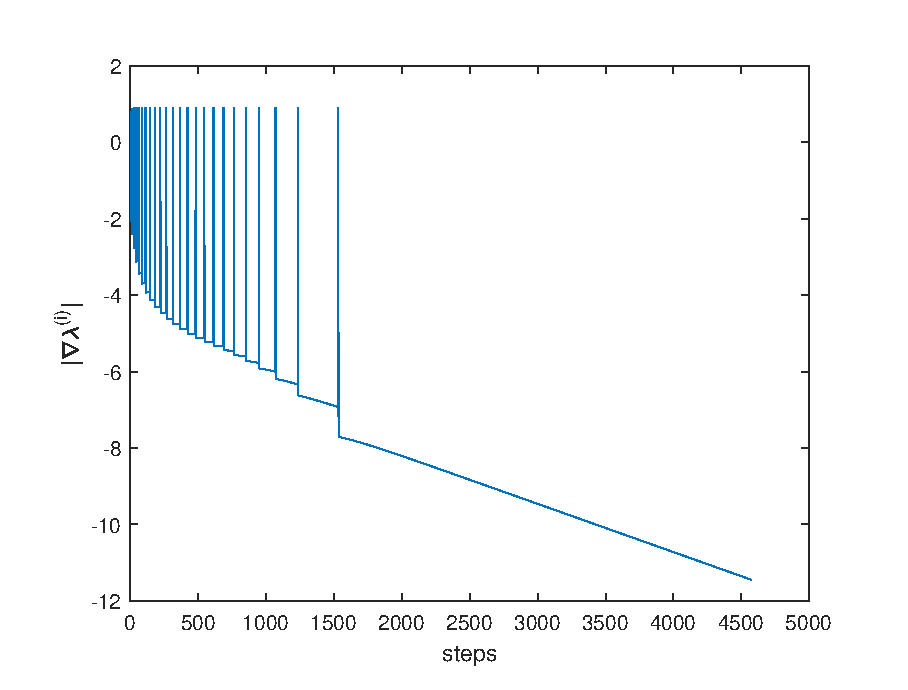
\includegraphics[width=0.4\textwidth]{1_100_lambda_origin_1.eps}}
            \subfloat[$n=101$]
            {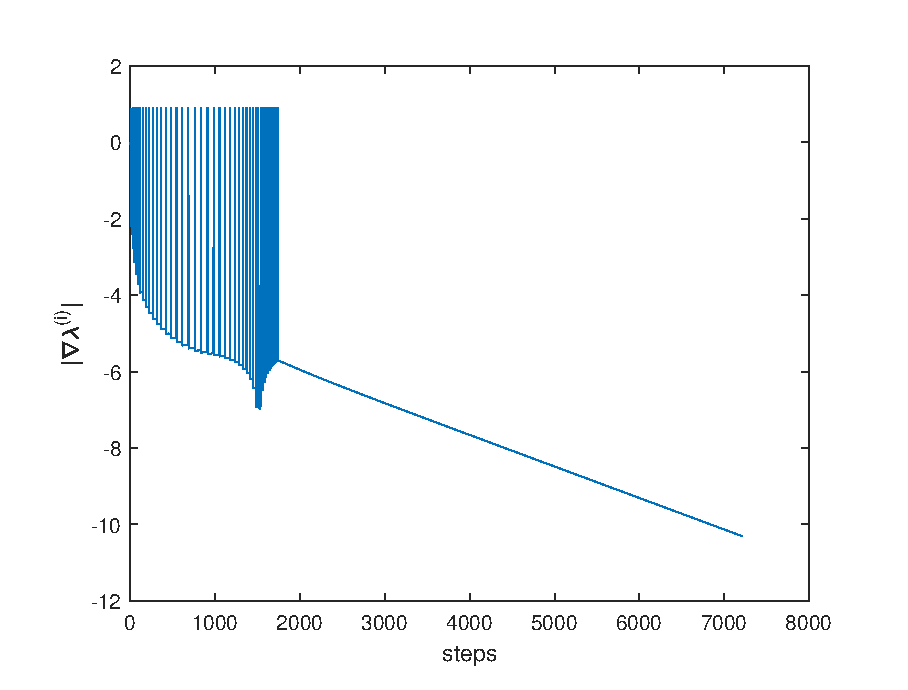
\includegraphics[width=0.4\textwidth]{1_101_lambda_origin_1.eps}}
            \caption{特征值误差曲线}
        \end{figure}
        \begin{figure}[htbp]
            \centering
            \subfloat[$n=100$]
            {\includegraphics[width=0.4\textwidth]{1_100_x_origin_1.eps}}
            \subfloat[$n=101$]
            {\includegraphics[width=0.4\textwidth]{1_101_x_origin_1.eps}}
            \caption{特征子空间距离曲线}
        \end{figure}
        \begin{figure}[htbp]
            \centering
            \subfloat[$n=100$]
            {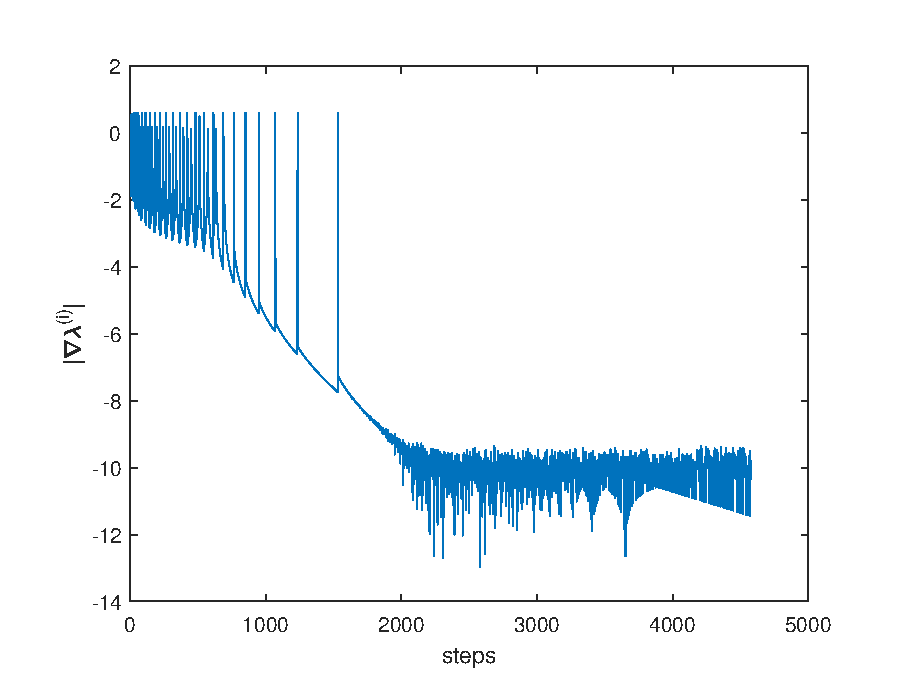
\includegraphics[width=0.4\textwidth]{1_100_lambda_atiken_1.eps}}
            \subfloat[$n=101$]
            {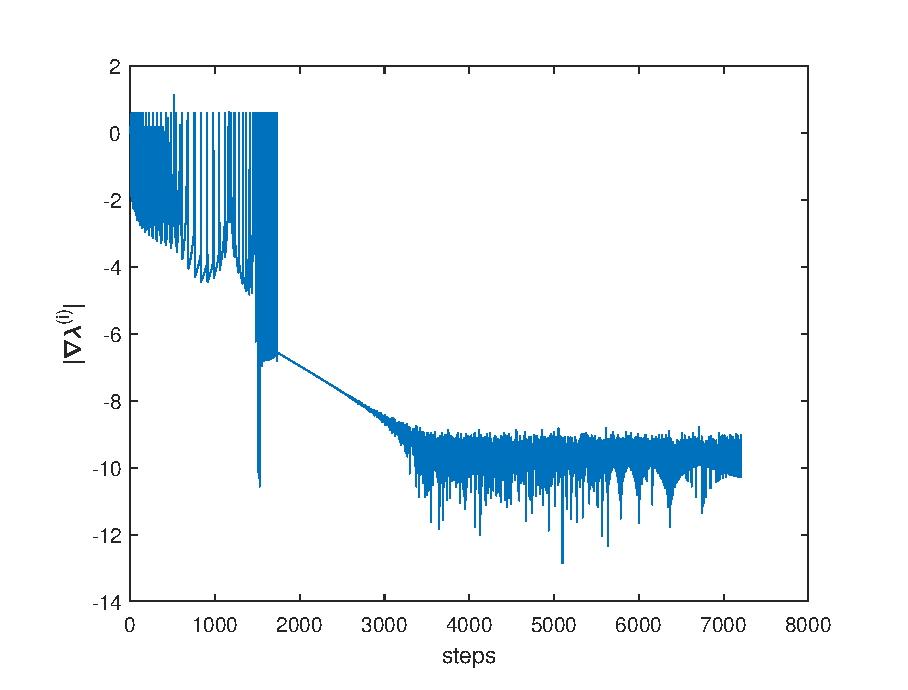
\includegraphics[width=0.4\textwidth]{1_101_lambda_atiken_1.eps}}
            \caption{使用Atiken加速的特征值误差曲线}
        \end{figure}
        \begin{figure}[htbp]
            \centering
            \subfloat[$n=100$]
            {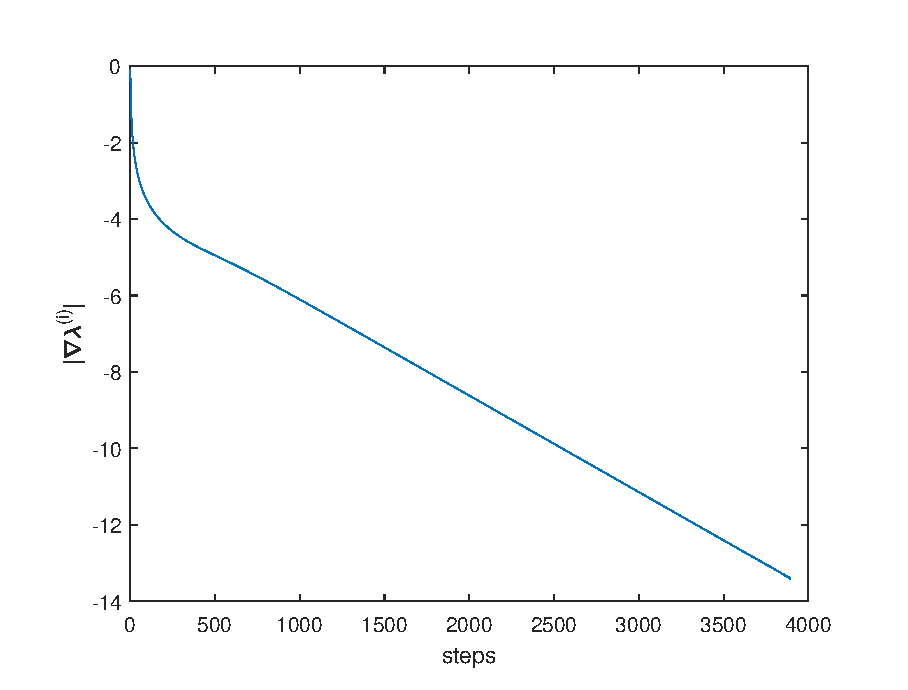
\includegraphics[width=0.4\textwidth]{1_100_lambda_rayleigh_1.eps}}
            \subfloat[$n=101$]
            {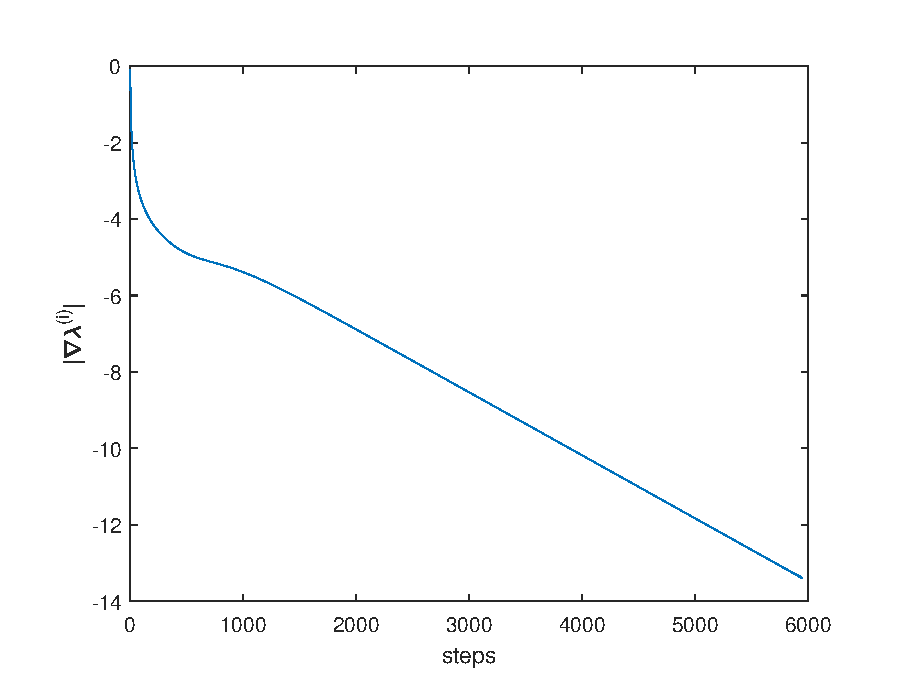
\includegraphics[width=0.4\textwidth]{1_101_lambda_rayleigh_1.eps}}
            \caption{使用Rayleigh商加速的特征值误差曲线}
        \end{figure}
        \par
        图象下界表明收敛速度约为线性图线,特征子空间距离下降到$10^{-8}$量级后下降受限。当$n=100$和$n=101$时,未采用任何加速技术的正幂法特征值相邻误差分别在约3500步和7000步达到$10^{-10}$量级,而应用Atiken加速技术后特征值相邻误差分别在约2000步和3500步达到$10^{-10}$量级,应用Rayleigh商加速技术后特征值相邻误差分别在约2000步和4000步达到$10^{-10}$量级。除此以外,Rayleigh商加速技术相邻误差稳定下降,未出现未采用任何加速技术和Atiken加速技术的震荡情形,在数值精度上达到$10^{-14}$,存在较大的优越性。
        \par
        \ 
        \par
        \ 
        \par
        将采用初始向量$v_0=[1,1,\dots,1]^{\mathrm{T}}$的上述幂法收敛最终特征信息结果与Matlab的\texttt{eig()}函数结果相比较,发现幂法实际收敛于矩阵$T_n$的次主特征信息
        $$
        \lambda_2=
        \begin{cases}
            3.99613119426719&,n=100 \\
            3.99620665747409&,n=101
        \end{cases}
        $$
        出现这种情况,考虑是初始特征向量在主特征值对应特征向量上的投影分量系数$\alpha_1=0$。改用$\tilde{v}_0=[0,1,\dots,1]^{\mathrm{T}}$重新执行正幂法和各加速技术,运行结果如Figure 5-8所示。

        \begin{figure}[htbp]
            \centering
            \subfloat[$n=100$]
            {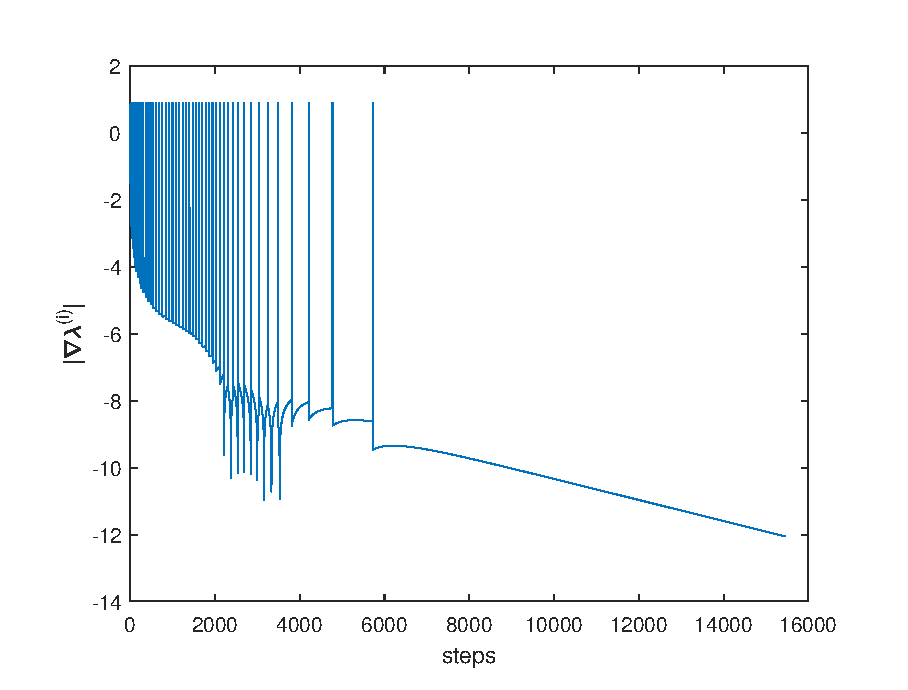
\includegraphics[width=0.4\textwidth]{1_100_lambda_origin_0.eps}}
            \subfloat[$n=101$]
            {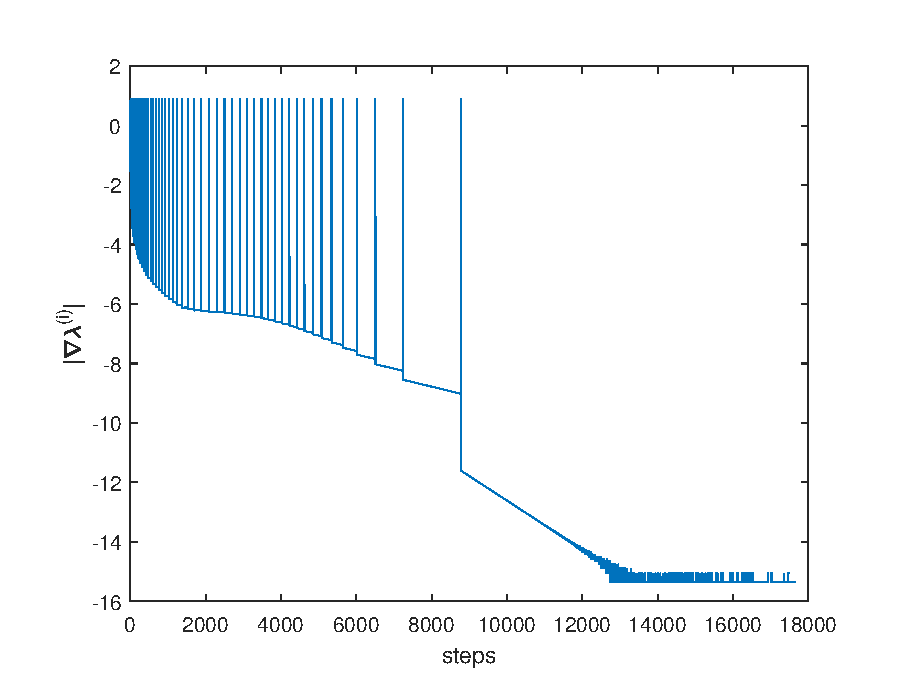
\includegraphics[width=0.4\textwidth]{1_101_lambda_origin_0.eps}}
            \caption{以$\tilde{v}_0=[0,1,\dots,1]^\mathrm{T}$为初始向量的特征值误差曲线}
        \end{figure}
        
        \begin{figure}[htbp]
            \centering
            \subfloat[$n=100$]
            {\includegraphics[width=0.4\textwidth]{1_100_x_origin_0.eps}}
            \subfloat[$n=101$]
            {\includegraphics[width=0.4\textwidth]{1_101_x_origin_0.eps}}
            \caption{以$\tilde{v}_0=[0,1,\dots,1]^\mathrm{T}$为初始向量的特征子空间距离曲线}
        \end{figure}
        
        \begin{figure}[htbp]
            \centering
            \subfloat[$n=100$]
            {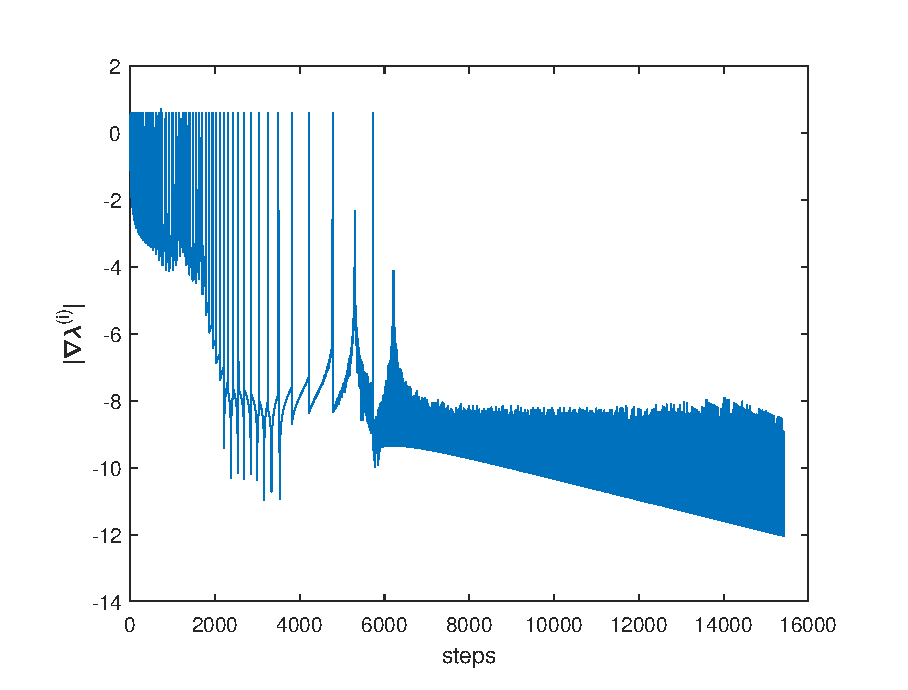
\includegraphics[width=0.4\textwidth]{1_100_lambda_atiken_0.eps}}
            \subfloat[$n=101$]
            {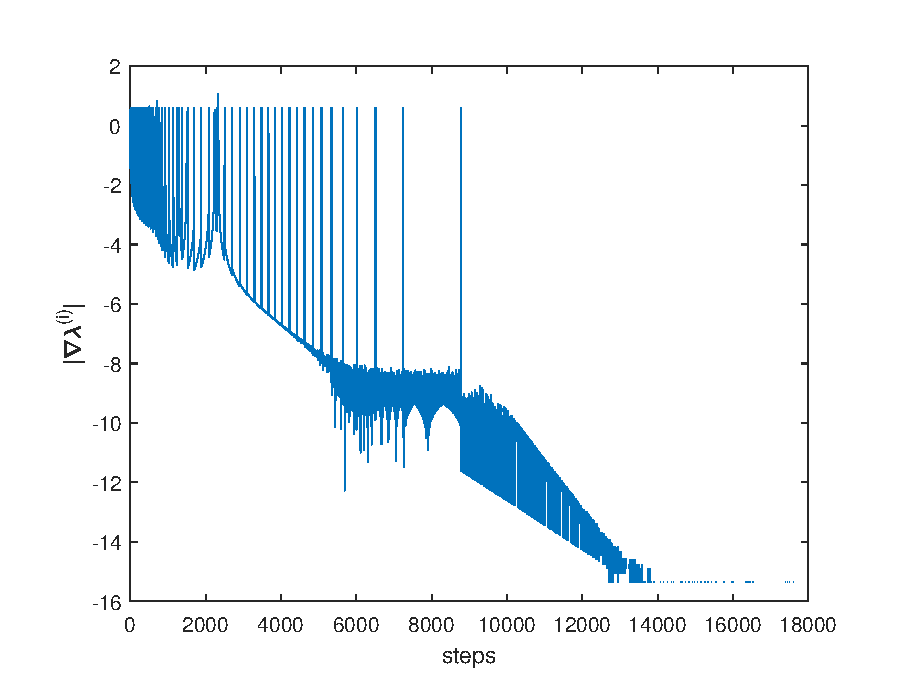
\includegraphics[width=0.4\textwidth]{1_101_lambda_atiken_0.eps}}
            \caption{以$\tilde{v}_0=[0,1,\dots,1]^\mathrm{T}$为初始向量并使用Atiken加速的特征值误差曲线}
        \end{figure}
        
        \begin{figure}[htbp]
            \centering
            \subfloat[$n=100$]
            {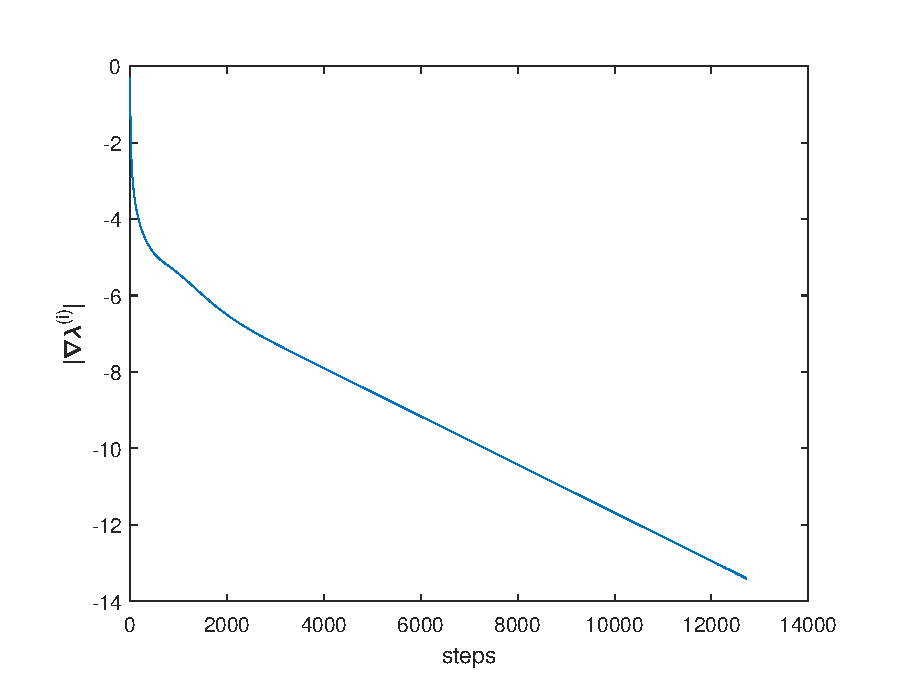
\includegraphics[width=0.4\textwidth]{1_100_lambda_rayleigh_0.eps}}
            \subfloat[$n=101$]
            {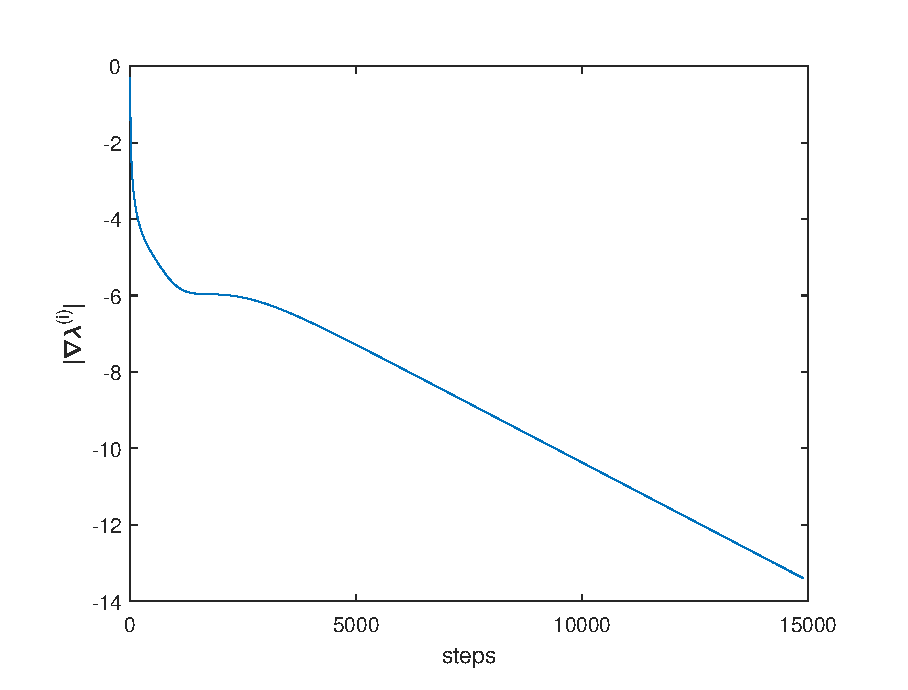
\includegraphics[width=0.4\textwidth]{1_101_lambda_rayleigh_0.eps}}
            \caption{以$\tilde{v}_0=[0,1,\dots,1]^\mathrm{T}$为初始向量并使用Rayleigh商加速的特征值误差曲线}
        \end{figure}

        \par
        各方法的迭代步数均变为原来的3倍左右。通过\texttt{eig()}函数获取$\left|\lambda_1\right|,\left|\lambda_2\right|,\left|\lambda_3\right|$,以$n=100$为例
        $$\left|\dfrac{\lambda_2}{\lambda_1}\right|\simeq0.9993$$
        $$\left|\dfrac{\lambda_3}{\lambda_2}\right|\simeq0.9988$$
        这表明收敛速度确实下降。最终收敛结果为矩阵$T_n$的主特征信息
        $$
        \lambda_1=
        \begin{cases}
            3.99903256458398&,n=100 \\
            3.99905143942673&,n=101
        \end{cases}
        $$
    \par
    \ 
    \par
    \ 
    \par
    下述各题特征值真值及其对应特征向量均以\texttt{[V,D]=eig()}给出的结果为参考值。
    \subsection{练习6.4.2}
        \par
        练习6.4.2的实验结果如Figure 9-12所示。

        \begin{figure}[htbp]
            \centering
            \subfloat[$q=2$]
            {\includegraphics[width=0.4\textwidth]{2_100_lambda_2.eps}}
            \subfloat[$q=3$]
            {\includegraphics[width=0.4\textwidth]{2_100_lambda_3.eps}}
            \caption{$n=100$的特征值误差曲线}
        \end{figure}
        
        \begin{figure}[htbp]
            \centering
            \subfloat[$q=2$]
            {\includegraphics[width=0.4\textwidth]{2_100_x_2.eps}}
            \subfloat[$q=3$]
            {\includegraphics[width=0.4\textwidth]{2_100_x_3.eps}}
            \caption{$n=100$的特征向量误差曲线}
        \end{figure}
        
        \begin{figure}[htbp]
            \centering
            \subfloat[$q=2$]
            {\includegraphics[width=0.4\textwidth]{2_101_lambda_2.eps}}
            \subfloat[$q=3$]
            {\includegraphics[width=0.4\textwidth]{2_101_lambda_3.eps}}
            \caption{$n=101$的特征值误差曲线}
        \end{figure}
        
        \begin{figure}[htbp]
            \centering
            \subfloat[$q=2$]
            {\includegraphics[width=0.4\textwidth]{2_101_x_2.eps}}
            \subfloat[$q=3$]
            {\includegraphics[width=0.4\textwidth]{2_101_x_3.eps}}
            \caption{$n=101$的特征向量误差曲线}
        \end{figure}
        \par
        由于矩阵阶数较低,且存在解大量同型方程组过程,程序调用第1章Crout分解代码\texttt{lu\_crout()}执行LU分解并将分解结果应用于每次迭代,降低了计算复杂度。在原点平移策略应用过程中,当$n=100$时反幂法顺利执行到底,当$n=101$时,\texttt{lu\_crout()}反馈出现了除零情形,这表明前$n-1$级顺序主子式不全为正,亦即矩阵$T_n-qI_n$非正定,即$\lambda=2$和$\lambda=3$皆为$T_n$的特征值。对$q$引入小扰动$\delta q=0.01$,重新执行反幂法求解对应的特征向量。
        \par
        在$n=100$的情形,当$q=3$时反幂法收敛到距离$q=3$最近的特征值$\lambda=2.98198816194664$及其对应特征向量。当$q=2$时,考虑到$T_n$的特征值关于$\lambda=2$对称分布,由此对反幂法作修正,即连续执行两步幂法,最终程序执行结果收敛到特征值
        $$
        \lambda_1=1.968896376044811
        $$
        $$
        \lambda_2=2.031103623955187
        $$
        及其特征向量。

    \subsection{练习6.4.3}
        \par
        练习6.4.3的实验结果如Figure 13所示,采用$n=101$和原点位移量$q=2.005$。在反幂法的前4步,特征值误差下降到$10^{-8}$量级,在第5步误差出现反弹,误差上升到$10^{-2}$量级并在5步内误差没有任何改善,在第11步才进一步下降并完成求解。

        \begin{figure*}[ht]
            \centering
            \includegraphics[width=14cm,height=10cm]{3.eps}
            \caption{反幂法“一次迭代”特性观察}
        \end{figure*}
        
    \subsection{练习6.4.4}
        \par
        练习6.4.4中使用收缩技术\texttt{deflation()}和同时迭代技术\texttt{iterate\_meanwhile\_method()}分别求解$n=100$和$n=101$的前两个特征值对应特征信息的对应误差如表1和表2所示。相比之下,除$n=101$的情形主特征值的计算,同时迭代方法均给出了比使用收缩技术更好的结果。

        \begin{table}[htbp]%调节图片位置,h:浮动;t:顶部;b:底部;p:当前位置
            \centering
            \label{tab:1}  
            \begin{tabular}{ccc}%表格中的数据居中,c的个数为表格的列数
                \hline\hline\noalign{\smallskip}	
                \  & \texttt{deflation()} & \texttt{iterate\_meanwhile\_method()} \\
                \noalign{\smallskip}\hline\noalign{\smallskip}
                $\left|\lambda_1-\lambda_1^*\right|$ & $1.21678400688552\times 10^{-9}$ & $4.44089209850063\times 10^{-16}$  \\
                $\mathrm{dist}(span\{x_1\},span\{x_1^*\})$ & $1.41421356234100$ & $1.49011611938477\times 10^{-8}$ \\
                $\left|\lambda_2-\lambda_2^*\right|$ & $1.75366050569892\times 10^{-8}$ & $4.44089209850063\times 10^{-16}$ \\
                $\mathrm{dist}(span\{x_2\},span\{x_2^*\})$ & $3.60965059486383\times 10^{-6}$ & $3.16101363831705\times 10^{-8}$ \\
                \noalign{\smallskip}\hline
            \end{tabular}
            \caption{$n=100$}
        \end{table}

        \begin{table}[htbp]%调节图片位置,h:浮动;t:顶部;b:底部;p:当前位置
            \centering
            \label{tab:1}  
            \begin{tabular}{ccc}%表格中的数据居中,c的个数为表格的列数
                \hline\hline\noalign{\smallskip}	
                \  & \texttt{deflation()} & \texttt{iterate\_meanwhile\_method()} \\
                \noalign{\smallskip}\hline\noalign{\smallskip}
                $\left|\lambda_1-\lambda_1^*\right|$ & $8.88178419700125\times 10^{-16}$ & $1.33226762955019\times 10^{-15}$  \\
                $\mathrm{dist}(span\{x_1\},span\{x_1^*\})$ & $9.93097275708284\times 10^{-6}$ & $0$ \\
                $\left|\lambda_2-\lambda_2^*\right|$ & $1.69141762818015\times 10^{-8}$ & $1.55431223447522\times 10^{-14}$ \\
                $\mathrm{dist}(span\{x_2\},span\{x_2^*\})$ & $1.41421356236822$ & $1.28318812643414\times 10^{-6}$ \\
                \noalign{\smallskip}\hline
            \end{tabular}
            \caption{$n=101$}
        \end{table}

    \subsection{练习6.4.5}
        \par
        练习6.4.5的实验结果如Figure 14-16所示。

        \begin{figure}[htbp]
            \centering
            \subfloat[$\left\|E_k\right\|_F$]
            {\includegraphics[width=0.4\textwidth]{5_classical_e.eps}}
            \subfloat[对角元收敛过程]
            {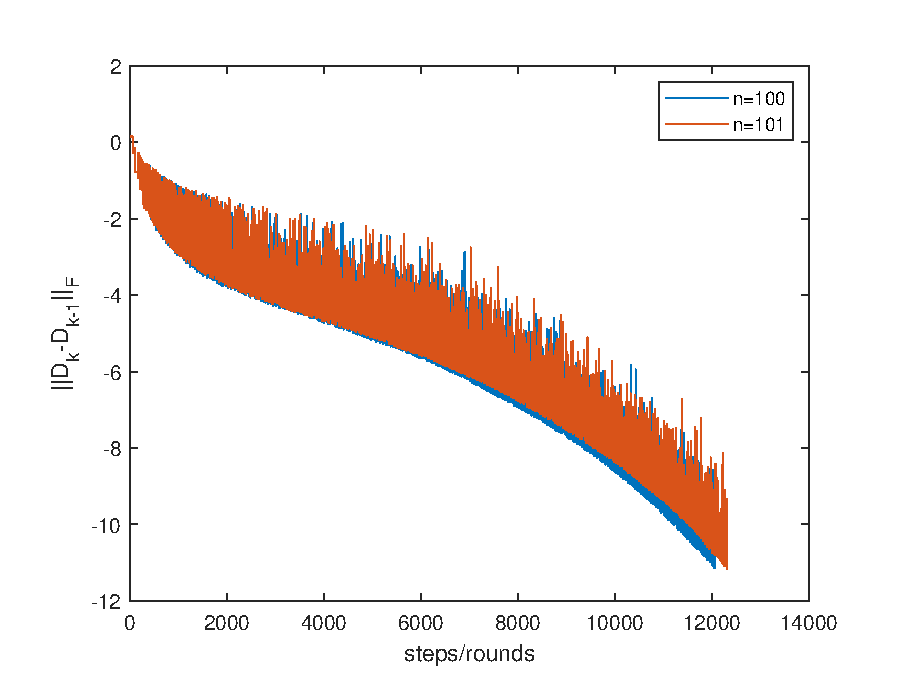
\includegraphics[width=0.4\textwidth]{5_classical_d.eps}}
            \caption{使用古典Jacobi方法求解全部特征值}
        \end{figure}
        
        \begin{figure}[htbp]
            \centering
            \subfloat[$\left\|E_k\right\|_F$]
            {\includegraphics[width=0.4\textwidth]{5_loop_e.eps}}
            \subfloat[对角元收敛过程]
            {\includegraphics[width=0.4\textwidth]{5_loop_d.eps}}
            \caption{使用循环Jacobi方法求解全部特征值}
        \end{figure}
        
        \begin{figure}[htbp]
            \centering
            \subfloat[$\left\|E_k\right\|_F$]
            {\includegraphics[width=0.4\textwidth]{5_threshold_e.eps}}
            \subfloat[对角元收敛过程]
            {\includegraphics[width=0.4\textwidth]{5_threshold_d.eps}}
            \caption{使用阈值Jacobi方法求解全部特征值}
        \end{figure}

        \par
        \ 
        \par
        \ 
        \par
        \ 
        \par
        \ 
        \par
        \ 
    \subsection{练习6.4.6}
        \par
        练习6.4.6的实验结果如下所示,其中Figure 17作出了各范围内特征值的误差曲线,表3和表4给出了\texttt{sturm()}最终迭代结果和\texttt{inverse\_method()}的结果误差比较,用户指标均取为$\epsilon=10^{-8}$。

        \begin{figure}[htbp]
            \centering
            \subfloat[$n=100$]
            {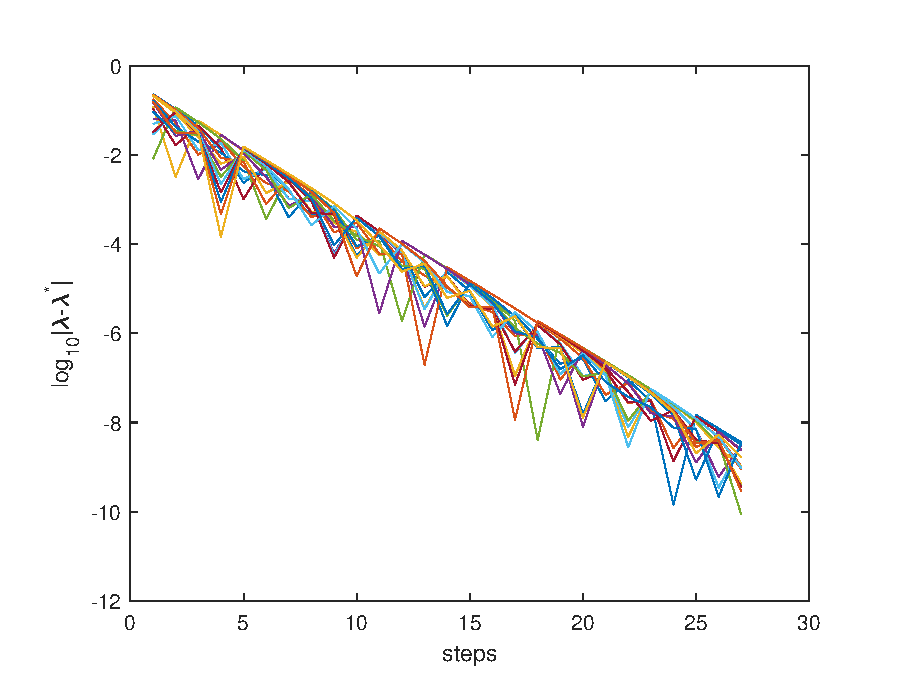
\includegraphics[width=0.4\textwidth]{6_100.eps}}
            \subfloat[$n=101$]
            {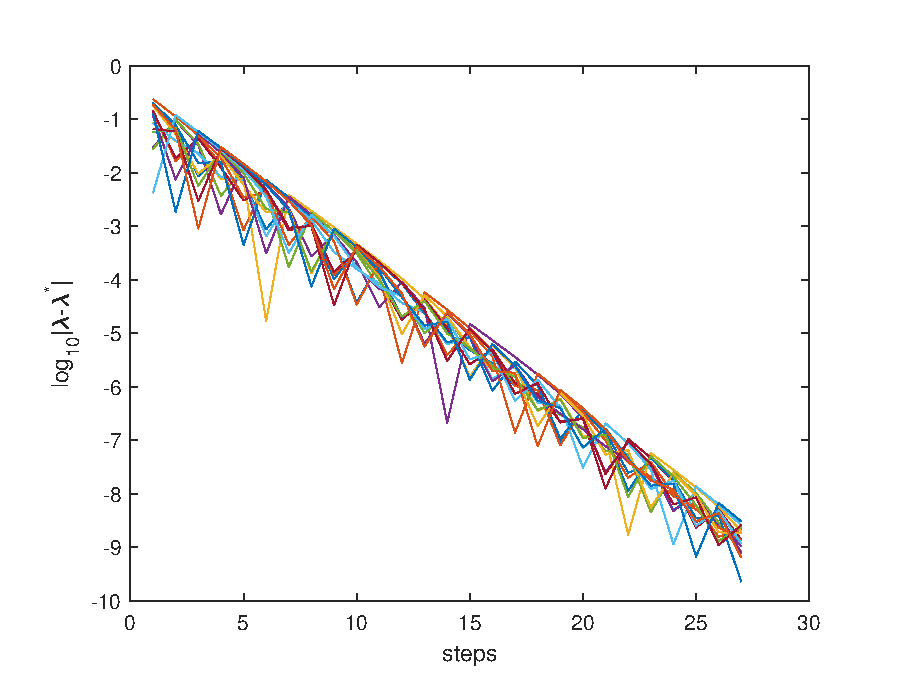
\includegraphics[width=0.4\textwidth]{6_101.eps}}
            \caption{使用Strum区间二分法的误差曲线}
        \end{figure}

        \begin{table}[h!]%调节图片位置,h:浮动;t:顶部;b:底部;p:当前位置
            \centering
            \label{tab:1}  
            \begin{tabular}{ccc}%表格中的数据居中,c的个数为表格的列数
                \hline\hline\noalign{\smallskip}	
                \  & \texttt{sturm()} & \texttt{inverse\_method()} \\
                \noalign{\smallskip}\hline\noalign{\smallskip}
                $\left|\lambda_1-\lambda_1^*\right|$ & $3.58093799057713\times 10^{-9}$ & $2.22044604925031\times 10^{-16}$ \\
                $\left|\lambda_2-\lambda_2^*\right|$ & $1.03601749401605\times 10^{-9}$ & $0$ \\
                $\left|\lambda_3-\lambda_3^*\right|$ & $1.01872599245212\times 10^{-9}$ & $2.22044604925031\times 10^{-16}$ \\
                $\left|\lambda_4-\lambda_4^*\right|$ & $3.12476866604072\times 10^{-9}$ & $0$ \\
                $\left|\lambda_5-\lambda_5^*\right|$ & $3.66601415890955\times 10^{-10}$ & $2.22044604925031\times 10^{-16}$ \\
                $\left|\lambda_6-\lambda_6^*\right|$ & $3.37994210397596\times 10^{-9}$ & $4.44089209850063\times 10^{-16}$ \\
                $\left|\lambda_7-\lambda_7^*\right|$ & $2.36138131270991\times 10^{-9}$ & $2.22044604925031\times 10^{-16}$ \\
                $\left|\lambda_8-\lambda_8^*\right|$ & $3.19904680523564\times 10^{-9}$ & $2.22044604925031\times 10^{-16}$ \\
                $\left|\lambda_9-\lambda_9^*\right|$ & $8.97356855489306\times 10^{-10}$ & $2.22044604925031\times 10^{-16}$ \\
                $\left|\lambda_{10}-\lambda_{10}^*\right|$ & $4.22189394555517\times 10^{-10}$ & $4.44089209850063\times 10^{-16}$ \\
                $\left|\lambda_{11}-\lambda_{11}^*\right|$ & $2.45831932588203\times 10^{-9}$ & $4.44089209850063\times 10^{-16}$ \\
                $\left|\lambda_{12}-\lambda_{12}^*\right|$ & $8.49618153608844\times 10^{-11}$ & $6.66133814775094\times 10^{-16}$ \\
                $\left|\lambda_{13}-\lambda_{13}^*\right|$ & $9.56702717047619\times 10^{-10}$ & $4.44089209850063\times 10^{-16}$ \\
                $\left|\lambda_{14}-\lambda_{14}^*\right|$ & $3.45895090347881\times 10^{-10}$ & $4.44089209850063\times 10^{-16}$ \\
                $\left|\lambda_{15}-\lambda_{15}^*\right|$ & $3.50817064287412\times 10^{-9}$ & $4.44089209850063\times 10^{-16}$ \\
                $\left|\lambda_{16}-\lambda_{16}^*\right|$ & $2.85622636653216\times 10^{-10}$ & $4.44089209850063\times 10^{-16}$ \\
                $\left|\lambda_{17}-\lambda_{17}^*\right|$ & $1.67239866399882\times 10^{-9}$ & $4.44089209850063\times 10^{-16}$ \\
                \noalign{\smallskip}\hline
            \end{tabular}
            \caption{$n=100$}
        \end{table}

        \begin{table}[htbp]%调节图片位置,h:浮动;t:顶部;b:底部;p:当前位置
            \centering
            \label{tab:1}  
            \begin{tabular}{ccc}%表格中的数据居中,c的个数为表格的列数
                \hline\hline\noalign{\smallskip}	
                \  & \texttt{sturm()} & \texttt{inverse\_method()} \\
                \noalign{\smallskip}\hline\noalign{\smallskip}
                $\left|\lambda_1-\lambda_1^*\right|$ & $1.19161858158634\times 10^{-9}$ & $4.44089209850063\times 10^{-16}$ \\
                $\left|\lambda_2-\lambda_2^*\right|$ & $2.15742979037259\times 10^{-9}$ & $2.22044604925031\times 10^{-16}$ \\
                $\left|\lambda_3-\lambda_3^*\right|$ & $2.00868432997936\times 10^{-9}$ & $4.44089209850063\times 10^{-16}$ \\
                $\left|\lambda_4-\lambda_4^*\right|$ & $1.04068687001302\times 10^{-9}$ & $2.22044604925031\times 10^{-16}$ \\
                $\left|\lambda_5-\lambda_5^*\right|$ & $8.25910229096394\times 10^{-10}$ & $2.22044604925031\times 10^{-16}$ \\
                $\left|\lambda_6-\lambda_6^*\right|$ & $2.59197485696916\times 10^{-9}$ & $4.44089209850063\times 10^{-16}$ \\
                $\left|\lambda_7-\lambda_7^*\right|$ & $1.39210931671130\times 10^{-9}$ & $2.22044604925031\times 10^{-16}$ \\
                $\left|\lambda_8-\lambda_8^*\right|$ & $2.25924390306886\times 10^{-10}$ & $2.22044604925031\times 10^{-16}$ \\
                $\left|\lambda_9-\lambda_9^*\right|$ & $1.35562272518541\times 10^{-9}$ & $0$ \\
                $\left|\lambda_{10}-\lambda_{10}^*\right|$ & $1.81810611010746\times 10^{-9}$ & $0$ \\
                $\left|\lambda_{11}-\lambda_{11}^*\right|$ & $7.81351205958458\times 10^{-10}$ & $0$ \\
                $\left|\lambda_{12}-\lambda_{12}^*\right|$ & $2.41364950248624\times 10^{-9}$ & $2.22044604925031\times 10^{-16}$ \\
                $\left|\lambda_{13}-\lambda_{13}^*\right|$ & $1.17985066161452\times 10^{-9}$ & $4.44089209850063\times 10^{-16}$ \\
                $\left|\lambda_{14}-\lambda_{14}^*\right|$ & $2.63077426509994\times 10^{-9}$ & $4.44089209850063\times 10^{-16}$ \\
                $\left|\lambda_{15}-\lambda_{15}^*\right|$ & $3.05353231588867\times 10^{-9}$ & $2.22044604925031\times 10^{-16}$ \\
                $\left|\lambda_{16}-\lambda_{16}^*\right|$ & $6.41288799840822\times 10^{-10}$ & $2.22044604925031\times 10^{-16}$ \\
                \noalign{\smallskip}\hline
            \end{tabular}
            \caption{$n=101$}
        \end{table}
        \par
        \ 
        \par
        \ 
        \par
        将\texttt{strum()}的用户指标减小,其计算精度并未提高,仍然保持在$10^{-9}$量级,并且当用户指标过小时,计算误差出现了反弹,这验证了区间二分法的用户指标不能设置过小,否则可能出现符号判断错误的技术要点。
        \par
        从表中明显可看出反幂法给出了精度高得多的特征值结果,误差均在$10^{-16}$量级,说明在实际求解特征值的过程中,可以采用较低的用户指标的Strum序列区间二分法给出特征值的估计值,以此为基准作带原点偏移的反幂法进一步求解高精度特征值结果。

    \subsection{练习6.4.8}
        \par
        练习6.4.8的实验结果如表5所示。\texttt{threshold\_jacobi}给出了满意的特征值计算结果,而\texttt{eig()}除了主特征值计算正确外,另外两个特征值都给出了错误的结果。

        \begin{table}[htbp]%调节图片位置,h:浮动;t:顶部;b:底部;p:当前位置
            \centering
            \label{tab:1}  
            \begin{tabular}{ccc}%表格中的数据居中,c的个数为表格的列数
                \hline\hline\noalign{\smallskip}	
                \  & \texttt{threshold\_jacobi()} & \texttt{eig()} \\
                \noalign{\smallskip}\hline\noalign{\smallskip}
                $\lambda_1$ & $1.00000000000000\times 10^{40}$ & $1.00000000000000\times 10^{40}$  \\
                $\lambda_2$ & $9.90000000000000\times 10^{19}$ & $3.96678784561050\times 10^{23}$ \\
                $\lambda_3$ & $0.981818181818182$ & $-8.10000843110587\times 10^{19}$\\
                \noalign{\smallskip}\hline
            \end{tabular}
            \caption{使用阈值Jacobi方法\texttt{threshold\_jacobi()}与Matlab中\texttt{eig()}函数计算结果比较}
        \end{table}
        
\section{小结}
    \par
    通过上述实验题,特征信息的求解问题综合了线性与非线性求解过程,不同的求解方法给出了精度不同的特征信息计算值,而不同的方法有其特别适用的计算手段,例如阈值Jacobi方法求解(绝对值)小特征值时具有优势,在实际问题中应当对特征值有理论上的估计后选用适当的方法计算。

    \begin{thebibliography}{99}  
        \bibitem{ref1}林成森. 数值计算方法(下册)[M]. 北京: 科学出版社, 2005.
    \end{thebibliography}
\end{document}
